\chapter{Mere za ocenjevanje uspešnosti klasifikatorjev}

Naslov tega poglavja je presplošen: omejili se bomo namreč na klasifikacijo. Še več, celotno poglavje smo v ta del predavanj umestili, da predstavimo eno samo tehniko: površino pod krivuljo ROC. A da do nje pridemo in se poglobimo v to, kaj ta površina sploh pomeni, moramo uvesti nekaj drugih, pomembnih mer za ocenjevanje uspešnosti klasifikatorjev. V tem poglavju tudi ne bomo govorili o postopkih za ocenjevanje uspešnosti, saj te (prečno preverjanje, izloči enega, in testiranje po metodi stremena) že poznamo.

\section{Tabela napak}

Predpostavimo, da je naš klasifikacijski problem binaren, torej da imamo dva razreda. Med njima izberemo pozitivni (ciljni) razred in negativni razred. Pozitivni razred je navadno razred, ki je povezan z študijem pojava, za katerega smo oblikovali učne podatke. Na primer, v medicini, kjer primerjamo zdrave osebke in osebke z določeno diagnozo bi bili slednji v ciljnem (pozitivnem) razredu. Ali pa pri industrijski aplikaciji, kjer želimo na podlagi meritev identificirati nezanesljive izdelke, so ti slednji pozitivni primeri oziroma pripadajo ciljnemu razredu.

Klasifikator, ki smo ga razvili na neki učni množici, bo na testni množici lahko pravilno razvrstil pozitiven primer (zadetek, angl. {\em true positive}), ali pa ga bo napačno razvrstil v negativni razred (pogrešek, angl. {\em false positive}). Za neciljni, negativni primer, bo lahko pravilno napovedal njegov razred (pravilna zavrnitev, angl. {\em true negative}) ali pa dal napačno napoved (napačno pozitiven, angl. {\em false positive}). Število takih pravilnih oziroma nepravilnih napovedi na testni množici lahko zberemo in prikažemo v tabeli napak, ki jo konceptualno kaže tabela~\ref{t:confusion-matrix}, njen konkretni primer na podatkih o volitvah senatorjev (slavni podatkovni nabor {\tt voting}) pa slika~\ref{f:confusion-matrix}. Podatke za tabelo napak smo pri slednjem sestavili s pomočjo prečnega preverjanja, kjer smo tabelo napak najprej pridobili na vsaki od testnih množic posebej, na koncu pa skupaj prikazali vsote posameznih celic za vse testne množice oziroma za celoten postopek prečnega preverjanja skupaj.

\begin{table}[htbp]
\caption{Tabela napak \angl{confusion matrix}.}
\label{t:confusion-matrix}
\begin{center}
\begin{tabular}{rcccc}
& & \multicolumn{2}{c}{Dejanska vrednost} \\ 
& & $+$ & $-$ \\
\cmidrule(r){3-4}
Napovedana & $+$ & True Positive ($TP$) & False Positive ($FP$) & $P'$ \\
vrednost & $-$ & False Negative ($FN$) & True Negative ($TN$) & $N'$ \\ \cmidrule(r){3-4}
& & $P$ & $N$ \\
\end{tabular}
\end{center}
\end{table}

\begin{figure}[htbp]
\begin{center}
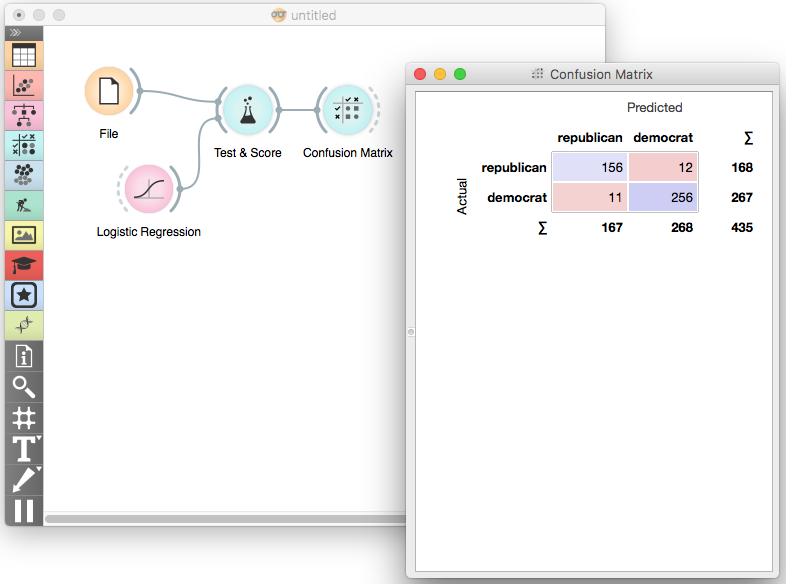
\includegraphics[width=12cm]{slike/tabela-napak-orange.png}
\caption{Shema za ocenjevanje in tabela napak v programu Orange.}
\label{f:confusion-matrix}
\end{center}
\end{figure}

Na osnovi tabele napak oziroma v njej predstavljenih števil pravilnih in napačnih napovedi lahko sestavimo nekaj mer, ki upoštevajo več celic v tabeli napak in s kombinacijo njih tvorijo smiselne ocene uspešnosti. Skupaj z samimi že opisanimi celicami tabele napak so te mere naslednje:
%
\begin{description}
\item[zadetek] ($TP$), število primerov v ciljnem razredu, pri katerih je bil napovedan pravilen razred \angl{true positive},
\item[pravilna zavrnitev]($TN$), število primerov negativnega razreda s točno napovedjo, \angl{true negative},
\item[napačno pozitiven, lažni alarm] ($FP$), število primerov v negativnem razredu, ki so bili napačno napovedani kot pozitivni, tudi napaka I. reda \angl{false positive},
\item[pogrešek] ($FN$), število primerov v negativnem razredu, ki so bili napačno prepoznani kot pozitivni primeri, tudi napaka II. reda \angl{false negative},
\item[občutljivost, priklic] \angl{sensitivity, true positive rate, recall}, $TPR = {TP / P} = {TP / (TP+FN)} $, delež pozitivnih primerov, ki smo jih pravilno napovedali oziroma jih pravilno priklicali,
\item[delež napačno pozitivnih, odpadek] (FPR), \angl{false positive rate, fall-out} $FPR = FP / N = FP / (FP + TN)$, delež napačno klasificiranih negativnih primerov,
\item[točnost] (ACC), \angl{accuracy}, $ACC = (TP + TN) / (P + N)$, delež primerov, za katere smo pravilno napovedali razred,
\item[specifičnost], stopnja pravilne zavrnitve (SPC), \angl{specificity, true negative rate}, $SPC = TN / N = TN / (FP + TN) = 1 - FPR$, dežel negativnih primerov, za katere smo pravilno napovedali razred,
\item[natančnost], delež pravilnih pozitivnih (PPV), \angl{positive predictive value, precision} $PPV = TP / (TP + FP)$, delež pravilno napovedanih pozitivnih primerov med vsemi pozitivnimi napovedi,
\item[delež pravilnih negativnih] (NPV), \angl{negative predictive value}, $NPV = TN / (TN + FN)$, delež pravilno napovedanih primerov med vsemi negativnimi primeri,
\item[mera F1] (F1) \angl{F1 score}, $F1 = 2\times(\frac{1}{\rm recall}+\frac{1}{\rm precision})^{-1}=$ je harmonično povprečje priklica in natančnosti.
\end{description}

Nekatere med zgornjimi merami so komplementarne; z optimizacijo (višanjem) ene od mer bomo zmanjšali vrednost druge. Na primer, če želimo zvišati priklic, nam je najbolj enostavno spustiti kriterij za klasifikacijo v pozitivni razred oziroma čim več primerov iz testne množice razglasiti za pozitivne. A bomo na ta način prav gotovo zmanjšali delež pravilnih pozitivnih napovedi. Podobno je s specifičnostjo in občutljivostjo: tudi tu za povečanje občutljivosti lahko spustimo mejo, ko primer razglasimo za pozitivnega, a bomo na ta način zmanjšali delež pravilno napovedanih negativnih primerov.

Zgornji kompromisi oziroma optimizacije izbranih mer na račun drugih so seveda pri strojnem učenju povezani s tem, da v praksi ne napovedujem razredov marveč njihove verjetnosti. Uporabljamo torej verjetnostne napovedi. Pri teh se moramo odločiti za prag oziroma vrednost, nad katero primeru določimo, da pripada ciljnemu razredu.

\subsection{Površina pod krivuljo ROC}

Prav posebna mera za ocenjevanje napovedne točnosti klasifikatorjev je površina pod krivuljo ROC \angl{area under receiving operator characteristics} in zato zasluži poseben razdelek. Mero so najprej uporabili tekom druge svetovne vojne in z njo skušali oceniti radariste ter njihovo točnost pri razlikovanju med zavezniškimi in agresorjevimi letali na radarskem zaslonu. Ocenjevali so jih v različnih pogojih (dopoldne, zvečer, po neprespani noči, ...) in ob različnih časih ter skušali, ne glede na njihovo stanje, radariste kar najbolj objektivno rangirati, od teh zelo uspešnih do drugih, ki so bolj često delali napake. Pri tem so opazili, da je uspešnost radaristov zelo odvisna od pogojev in psihofizičnega stanja, in da je posamezne meritve uspešnosti med seboj zelo težko primerjati.

Denimo, da so vsakič beležili nekaj, recimo okoli dvajset, poskusov prepoznave agresorjevih letal, in za dva radarista zabeležili priklic ($TPR$) in delež napačno pozitivnih napovedi ($FPR$) kot prikazuje tabela~\ref{t:radarista}. Meritve lahko prikažemo v grafu (slika~\ref{f:radarista}). Želimo, da bi $TPR$ bil čim višji in $FPR$ čim manjši. Meritve, ki segajo proti zgornjem levem kotu grafa so zato najbolj zaželene. Vidimo, da so rezultati radarista B boljši, saj njihova Paretto optimalna fronta prekrije Paretto optimalno fronto radarista B. Z drugimi besedami, konveksna ovojnica meritev za radarista B je levo in nad konveksno ovojnico radarista A.

\begin{table}[btp]
  \caption{Rezultati meritev uspešnosti dveh radaristov, kjer so uspešnost pri prvem (leva tabela) merili pri petih različnih pogojih in pri drugem (tabela na desni) pri štirih različnih pogojih.}
  \label{t:radarista}
  \centering{
    \belowbaseline[0pt]{
    \begin{tabular}{ccc}
      \toprule
      \# & $FPR$ & $TPR$ \\
      \midrule
      1 & 0.20 & 0.20 \\
      2 & 0.25 & 0.30 \\
      3 & 0.40 & 0.60 \\
      4 & 0.70 & 0.80 \\
      5 & 0.90 & 0.85 \\
      \bottomrule
    \end{tabular}}
    \hspace*{1cm}
    \belowbaseline[0pt]{
    \begin{tabular}{ccc}
      \toprule
      \# & $FPR$ & $TPR$ \\
      \midrule
      1 & 0.10 & 0.15 \\
      2 & 0.20 & 0.40 \\
      3 & 0.50 & 0.80 \\
      4 & 0.95 & 0.95 \\
      \bottomrule
    \end{tabular}}
  }
\end{table}

\begin{figure}[htbp]
\begin{center}
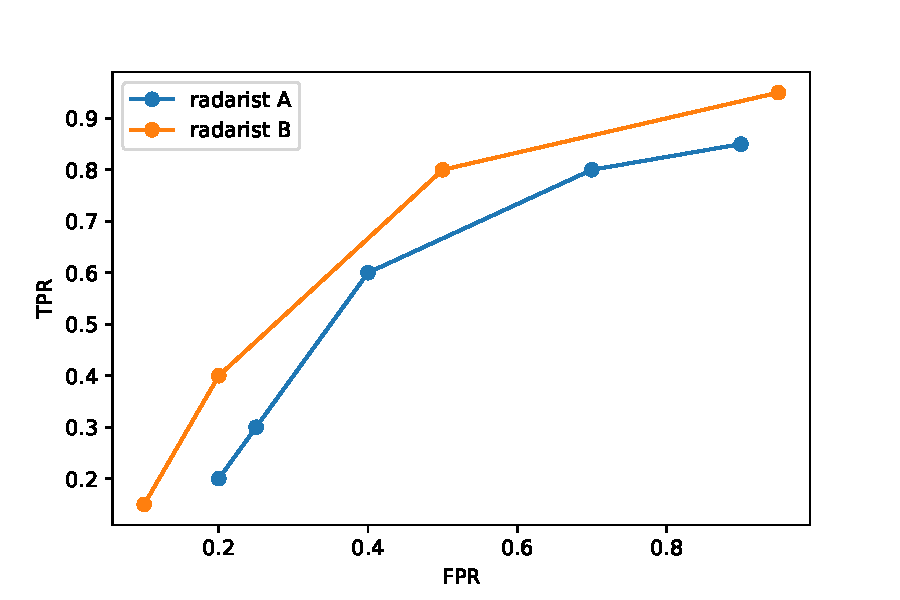
\includegraphics[width=9cm]{slike/radarista.pdf}
\caption{Krivulja ROC za rezultate meritev radaristov A in B iz tabele~\ref{t:radarista}.}
\label{f:radarista}
\end{center}
\end{figure}

Krivuljo ROC so ponovno odkrili v 1970-ih in jo najprej uporabljali v radiologiji~\cite{Hanley1982}, kasneje pa na celotnem področju medicine~\cite{Beck1986}. Da bi jo potem znova odkrili na prelomu stoletja in pričeli množično uporabljati na celotnem področju statistike in odkrivanja znanj iz podatkov.

Na enostavnem primeru si oglejmo si najprej konstrukcijo krivulje ROC, s katero opišemo rezultate testiranja izbranega postopka za strojno učenje. Denimo, da smo že zgradili model uvrščanja in bi radi ocenili njegovo točnost na testnih primerih. Naš klasifikacijski problem je dvovrednostni, napovedni model pa zna napovedati verjetnosti ciljnega razreda $p(y=1|{\bm x})$, kjer je ${\bm x}$ atributno opisan primer.

\begin{table}[htbp]
\caption{Testni primeri z dejanskim razredom in verjetnostjo za razred ``1'', kot jo je predlagal napovedni model, katerega točnost ocenjujemo. Primeri so urejeni skladno z napovedano verjetnostjo.}
\label{t-auc}
\begin{center}
\begin{tabular}{cc}
\toprule
$y$ & $p(y=1|X)$ \\
\midrule
1 & 0.89 \\
1 & 0.80 \\
1 & 0.80 \\
0 & 0.80 \\
1 & 0.63 \\
0 & 0.33 \\
1 & 0.33 \\
0 & 0.10 \\
0 & 0.10 \\
0 & 0.10 \\
\bottomrule
\end{tabular}
\end{center}
\end{table}

Točnost uvrščanja primerov s tabele~\ref{t-auc} je odvisna od praga verjetnosti $T$, nad katerimi bomo razglasili, da primeri pripadajo pozitivnemu razredu. Pri tem bomo opazovali $TPR$, to je delež pravilno napovedanih pozitivnih primerov med vsemi dejansko pozitivnimi \angl{true positive rate}, in $FPR$, delež negativnih primerov, za katere je bila napoved napačna \angl{false positive rate}. Izrazimo ti dve meri še z notacijo iz prejšnjega razdelka:
$$ TPR = {TP \over P} $$
$$ FPR = {FP \over N} $$

Vzemimo, da vse primere razglasimo kot pozitivne ($T<0.10$). Na ta način smo pravilno ``ulovili'' vse dejansko pozitivne primere in s tem dosegli najvišji delež pravilno napovedanih pozitivnih primerov med vsemi dejansko pozitivni primeri ($TP=P$, $TPR=1.0$). Tudi $FPR$ je s tem maksimalni, 1.0, saj smo vse negativne primere napačno uvrstili med pozitivne.

Drugače pa je, če vse primere iz testne razglasimo kot negativne ($T>0.89$). Primerov, ki bi jih razglasili za pozitivne, ni, zato $TPR=0$ in $FPR=0$.

Vse ostale vrednosti $TPR$ in $FPR$ bodo, za prag, ki ga izberemo med zgornjima dvema skrajnima mejama, nekje med 0 in 1. Najbolj zaželen prag bi bil tam, kjer bi vse razvrstitve v pozitivni razred bile pravilne in nobena ne bi bila nepravilna. V tej točki bi bil $TPR=1$ in $FPR=0$. Ali za naš primer taka vrednost praga obstaja?

Preskusimo sedaj vse možne mejne vrednosti $T$, kjer bi se nam vrednosti $TPR$ in $FPR$ lahko spremenile. Za naše podatke imamo štiri intervale, kjer lahko poiščemo take meje. Med 0.89 in 0.80, med 0.80 in 0.63, med 0.63 in 0.33, in med 0.33 in 0.10. Kje v teh intervalih bo dejansko naša mejna vrednost ni pomembno. Za te štiri meje izračunajmo sedaj vrednosti $TPR$ in $FPR$ in te vnesimo v graf (slika~\ref{f-roc}).

\begin{figure}[htbp]
\begin{center}
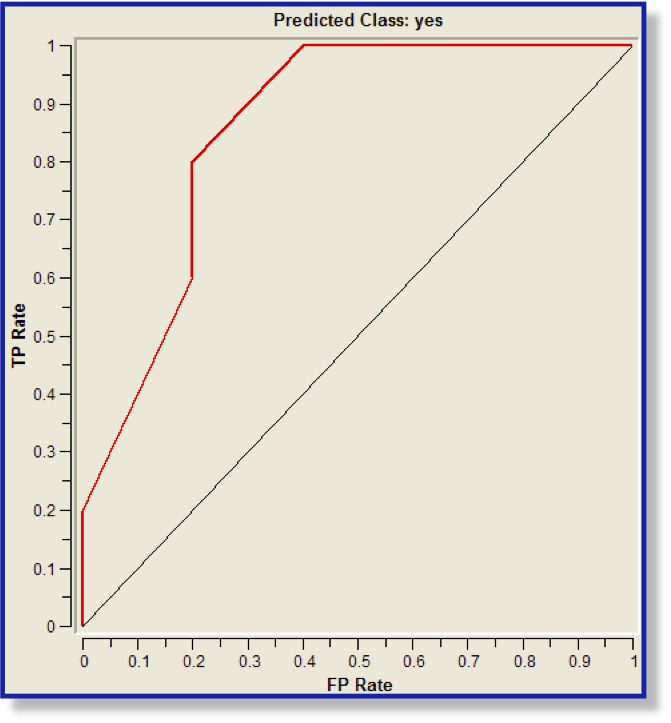
\includegraphics[width=7cm]{slike/roc.png}
\caption{Krivulja ROC za podatke s tabele~\ref{t-auc}.}
\label{f-roc}
\end{center}
\end{figure}

Obstaja tudi hitrejši način izrisa krivulja $ROC$, ki zahteva ureditev primerov po napovedani verjetnosti ciljnega razreda (kot smo to storili v tabeli~\ref{t-auc}). Postopek je naslednji:
%
\begin{enumerate}
\item Izrišemo graf z mrežo $1/N$ horizontalno in $1/P$ vertikalno.
\item Uredimo primere v seznam $L$ po padajoči verjetnosti napovedi v ciljni razred.
\item Pričnimo v točki (0,0).
\item Izberimo in iz seznama $L$ izključimo primere z najvišjo napovedano verjetnostjo. Naj ti primeri vključujejo $n_+$ primerov iz pozitivnega razreda, in $n_-$ primerov iz negativnega razreda. V mreži grafa se premaknimo $n_+$ razdelkov navzgor in $n_-$ razdelkov desno.
\item Če $L$ ni prazen, skoči na korak 4, sicer končaj.
\end{enumerate}

\begin{figure}[htbp]
\begin{center}
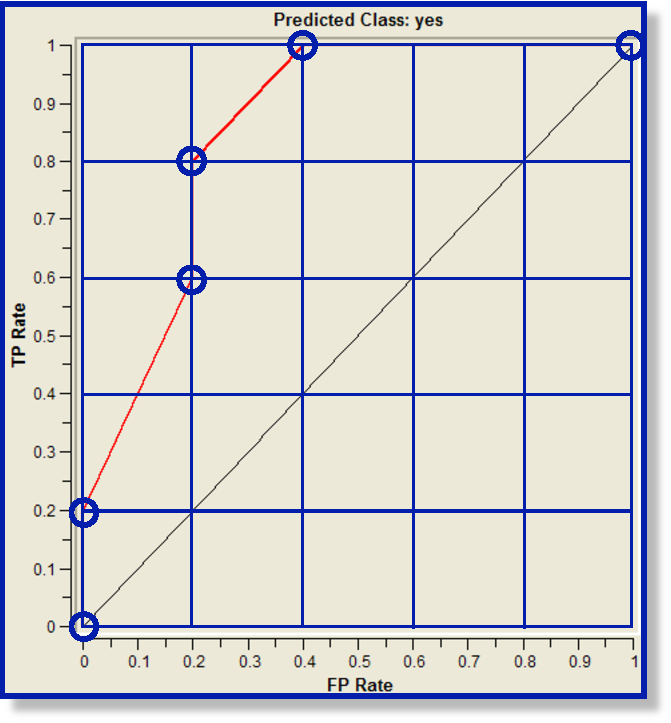
\includegraphics[width=7cm]{slike/roc-walk.pdf}
\caption{Mreža za izris krivulje ROC in sprehod po njenih točkah skladno s primeri s tabele~\ref{t-auc}.}
\label{f-roc-walk}
\end{center}
\end{figure}

Opazimo, da zgoraj opisan algoritem pravilno razpozna obe meri $TPR$ in $FPR$ za vse možne vrednosti praga verjetnosti (slika~\ref{f-roc-walk}).

Površino pod krivuljo ROC označimo z $AUC$. Pri naključnih napovedih pričakujemo, da bodo v obhodu zgornjega algoritma šli približno po diagonali grafi in bo $AUC=0.5$. To je tudi spodnja meja za to mero in je karakteristična za neuspešen napovedni model. Dejansko je meja za uspešne modele tipično pri $AUC=0.75$, modeli, ki imajo visoko napovedno točnost, pa imajo $AUC$ nekje nad $0.9$~\cite{Hanley1982}.

Površina pod ROC krivuljo pa ima še eno zanimivo lastnost. Če opazujemo sprehod po mreži za izris ROC krivulje, opazimo, da površina pod vsakem segmentom ravno ustreza številu napačno razvrščenih primerov, katerih verjetnost pozitivnega razreda je nad določeno mejo. Iz tega tudi sledi, da lahko $AUC$ izračunamo z enkratnim sprehodom skozi seznam primerov, ki je urejen glede na napovedano verjetnost ciljnega razreda. Mera $AUC$ ustreza verjetnosti, da za naključno izbrani primer ${\bm x}^+$ iz pozitivnega razreda in naključno izbrani primer ${\bm x}^-$ iz negativnega razreda velja $p(y=1|{\bm x}^+) > p(y=1|{\bm x}^-)$.

ROC krivuljo lahko rišemo in površino pod njo računamo za binarne klasifikatorje. Ko je razredov več, je potrebno večrazredni problem pretvoriti v dvorazrednega. Mero $AUC$ lahko potem računamo tako, da vsak element vektorja napovedanih verjetnosti razredov smatramo za svojo napoved, kjer je pozitivni razred samo tisti z ustrezno vrednostjo razreda in so vse ostale verjetnosti povezane z negativnim razredom. Ta pristop imenujemo mikro povprečenje~\angl{micro-averaging}. Pri drugačnem pristopu pa obravnavamo večrazredno klasifikacijo kot sprego binarnih klasifikatorjev tip eden-proti-ostalim, ter za vsakega posebej izračunamo $AUC$ oziroma krivulje ROC ter te povprečimo (t.im. makro povprečenje, angl. {\em macro-averagining}).

